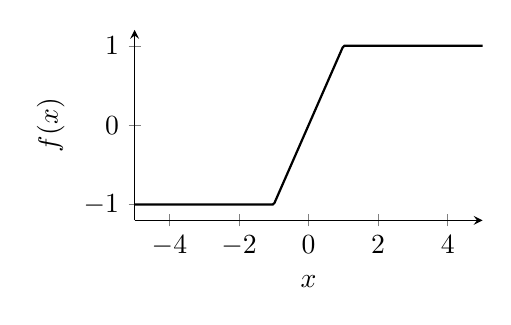
\begin{tikzpicture}
    \begin{axis}[
    axis lines=left,
    ymin=-1.2, ymax=1.2,
    xmin=-5, xmax=5,
    samples=200,
    domain=-5:5,
    width=6cm, height=4cm,
    xlabel={$x$}, ylabel={$f(x)$}
    ]
    \addplot[black,thick]{x <= -1 ? -1 : (x >= 1 ? 1 : x)};
    \end{axis}
\end{tikzpicture}